
    \centering
% \tikzsetnextfilename{conj_elemental1_R3}
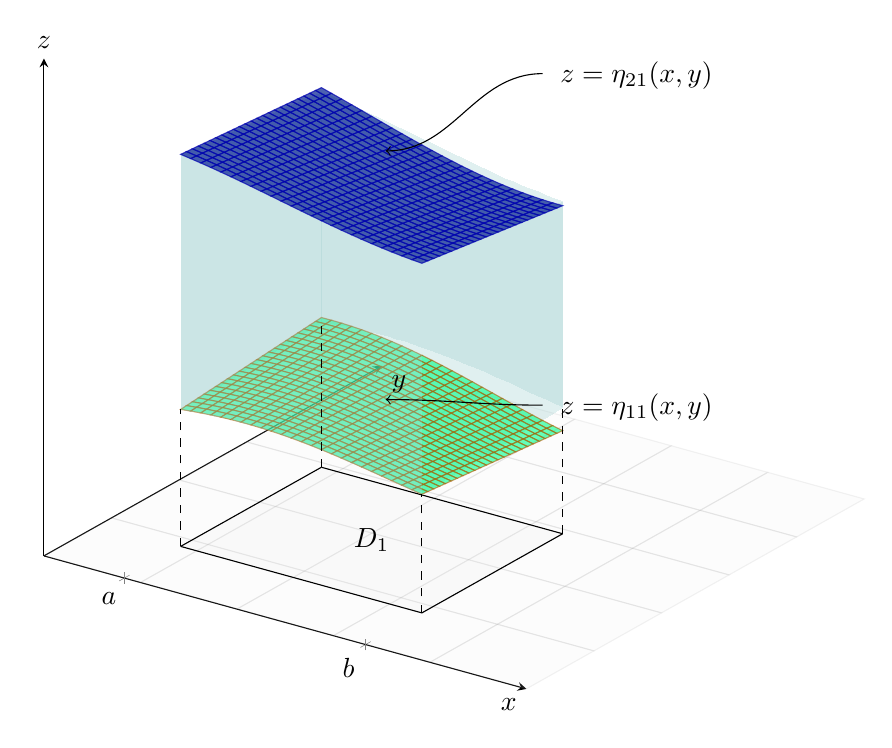
\begin{tikzpicture}
    \begin{axis}[
        view={35}{25}, % Ángulo de perspectiva
        width=12cm, height=12cm,
        grid=none,
        axis lines=center,
        xmin=0, xmax=6,
        ymin=0, ymax=6,
        zmin=0, zmax=6,
        xtick={1,4}, xticklabels={$a$,$b$}, % Marcas exactas de a y b en el eje x
        ytick=\empty, ztick=\empty,
        xlabel={$x$}, ylabel={$y$}, zlabel={$z$},
        every axis x label/.style={at={(ticklabel* cs:1)},anchor=north east},
        every axis y label/.style={at={(ticklabel* cs:1)},anchor=north west},
        every axis z label/.style={at={(ticklabel* cs:1)},anchor=south},
        clip=false
    ]

    % --- 0. Grilla en el piso (z=0) ---
    \addplot3 [surf, domain=0:6, domain y=0:6, samples=6, samples y=6, opacity=0.1, point meta=0, colormap={fondogris}{color=(gray!25) color=(gray!25)}, shader=faceted, faceted color=gray] (x,y,0);

    % --- 1. Dominio D_1 en R2 (Plano z=0) ---
    \addplot3 [surf, domain=1:4, domain y=0:1, samples=30, opacity=0.15, colormap={gray}{color=(gray!15) color=(gray!15)}, shader=interp, draw=none] 
        (x, {1 + 2.5*y}, 0);

    % Contorno de D1 (borde recto, uniendo las esquinas de la sombra)
    \draw[thin, black] (1, 1, 0) -- (4, 1, 0);
    \draw[thin, black] (1, 3.5, 0) -- (4, 3.5, 0);
    \draw[thin, black] (1, 1, 0) -- (1, 3.5, 0);
    \draw[thin, black] (4, 1, 0) -- (4, 3.5, 0);

    % --- 2. Paredes laterales (Efecto sólido) ---
    % Pared trasera
    \addplot3 [surf, domain=1:4, domain y=0:1, samples=30, opacity=0.3, colormap={teal}{color=(teal!40) color=(teal!40)}, shader=interp, draw=black!70] 
        (x, 3.5, { (1-y)*(1.5 + 0.2*sin(x*50) + 0.1) + y*(4.5 + 0.3*cos(x*40) - 0.2) });

    % Pared izquierda (en x=a)
    \addplot3 [surf, domain=0:1, domain y=0:1, samples=5, opacity=0.3, colormap={teal}{color=(teal!40) color=(teal!40)}, shader=interp, draw=black!70] 
        (1, {1 + 2.5*x}, { (1-y)*(1.5 + 0.2*sin(50) + 0.1*x) + y*(4.5 + 0.3*cos(40) - 0.2*x) });

    % Pared derecha (en x=b)
    \addplot3 [surf, domain=0:1, domain y=0:1, samples=5, opacity=0.3, colormap={teal}{color=(teal!40) color=(teal!40)}, shader=interp, draw=black!70] 
        (4, {1 + 2.5*x}, { (1-y)*(1.5 + 0.2*sin(200) + 0.1*x) + y*(4.5 + 0.3*cos(160) - 0.2*x) });

    % --- 3. Tapas del sólido ---
    % ¡AHORA SÍ!: Tapa inferior forzada a NARANJA plano con un mapa de color puro
    \addplot3 [surf, domain=1:4, domain y=0:1, samples=25, opacity=0.6, 
               colormap={pureorange}{rgb255=(0,255,140,0) rgb255=(1,255,140,0)}, shader=flat, draw=orange!70!black] 
        (x, {1 + 2.5*y}, { 1.5 + 0.2*sin(x*50) + 0.2*y*cos(x*40) });
        
    % Pared frontal
    \addplot3 [surf, domain=1:4, domain y=0:1, samples=30, opacity=0.3, colormap={teal}{color=(teal!40) color=(teal!40)}, shader=interp, draw=black!70] 
        (x, 1, { (1-y)*(1.5 + 0.2*sin(x*50)) + y*(4.5 + 0.3*cos(x*40)) });

    % Tapa superior forzada a AZUL plano con su propio mapa puro
    \addplot3 [surf, domain=1:4, domain y=0:1, samples=25, opacity=0.7, 
               colormap={pureblue}{rgb255=(0,30,144,255) rgb255=(1,30,144,255)}, shader=flat, draw=blue!70!black] 
        (x, {1 + 2.5*y}, { 4.5 + 0.3*cos(x*40) - 0.3*y*sin(x*30) });

    % --- 4. Esquinas y proyecciones (Líneas punteadas de soporte) ---
    \draw[dashed, thin] (1, 1, 0) -- (1, 1, {1.5 + 0.2*sin(50)});
    \draw[dashed, thin] (4, 1, 0) -- (4, 1, {1.5 + 0.2*sin(200)});
    \draw[dashed, thin] (1, 3.5, 0) -- (1, 3.5, {1.5 + 0.2*sin(50) + 0.1});
    \draw[dashed, thin] (4, 3.5, 0) -- (4, 3.5, {1.5 + 0.2*sin(200) + 0.1});

    % --- 5. Etiquetas ---
    \node at (2.5, 2.25, 0) {$D_1$};

    % Etiquetas de las superficies
    \node[anchor=west] at (3.5, 4, 5.2) {$z = \eta_{21}(x,y)$};
    \node[anchor=west] at (3.5, 4, 1.2) {$z = \eta_{11}(x,y)$};
    
    % Flechas a las superficies
    \draw[->, out=180, in=0, thin] (3.4, 4, 5.2) to (2.5, 2.5, 4.6);
    \draw[->, out=180, in=0, thin] (3.4, 4, 1.2) to (2.5, 2.5, 1.6);

\end{axis}
\end{tikzpicture}
\caption{Conjunto elemental de Tipo I.}
